\documentclass{ctexart}
\usepackage{amsmath}
\usepackage{amsfonts}
\def\vec#1{\mathbf{#1}}
\begin{document}
\title{计算物理作业18}
\author{刘畅\quad PB09203226}
\maketitle
{\bf[作业18]}: 调研一篇用分子动力学方法进行模拟计算的文献, 
综述你对文中采用的原理、算法、初始条件、可能的步骤和
结果的理解. 
\bigbreak
我调研的文献是 Alder, B.~J.; T.~E. Wainwright (1959), ``Studies in Molecular Dynamics. I. General Method'', {\sl J. Chem. Phys}. {\bf 31} (2): 459. 原文在
\verb|JChemPhys_31_459.pdf|. 这篇文章讨论了如何数值地
求解运动方程来计算几百个相互作用的经典粒子的运动轨迹, 之后还分析了
这种数值方法的局限性, 讨论了影响计算效率的几点因素, 最后讨论了
在统计物理学中的应用. 

\section{原理}
分子动力学方法的基本原理是数值地积分牛顿运动方程. 对于一个 $N$
体问题, $N$ 在 100 的数量级时, 既没有办法解析地求解牛顿方程, 
也没有办法直接套用统计力学的规律(由于 $N$ 不够大), 因此借助
计算机数值求解运动方程是唯一可行的办法. 

数值积分牛顿方程有一套通用的算法, 首先要给定系统的初始条件, 
例如所有分子的初始位形 $\vec r_i$ 和速度 $\vec v_i$, 然后选择一个小的时间间隔 $\Delta t$. 在每一个时刻 $t$, 都计算
分子间的相互作用力 $\vec F_i = -\nabla_i V(\vec r_i)$,
得到每个分子的加速度 $\vec a_i = \vec F_i/m$. 在接下来的
$\Delta t$ 时间里, 分子按照初速度为 $\vec v_i$, 加速度
为 $\vec a_i$ 的匀加速运动运行. 算法重复充分多次直到满意为止. 

\section{算法(具体的步骤)}
这篇文献中假设的分子间相互作用为方势井 (square-well potential):
\begin{equation}\label{potential}
V = \begin{cases}
\infty&\quad r<\sigma_1\\
V_0&\quad \sigma_1<r<\sigma_2\\
0&\quad r>\sigma_2
\end{cases}
\end{equation}
其中 $V_0$, $\sigma_1$, $\sigma_2$ 是常数.

算法首先设定初始位形(在后面的一节讨论), 然后计算系统出现
首次碰撞的时间 $t$. 这里碰撞指的是分子间距离达到 $\sigma_1$
或 $\sigma_2$, 这样按照上面的势能曲线, 分子间就会有吸引或排斥. 文献中推导了, 对分子 $i$ 和 $j$, 这个时间 $t_{ij}$ 由
\[
t^{(\alpha)}_{ij} = \frac{-b_{ij}\pm\left(b_{ij}^2
-u_{ij}^2C^{(\alpha)}_{ij}\right)^{1/2}}{u^2_{ij}}
\]
给出, 其中
\begin{align}\label{cond}
\vec r_{ij} = \vec r_{i0}-\vec r_{j0}\qquad&
b_{ij} = \vec r_{ij} \cdot \vec u_{ij}\\
\vec u_{ij} = \vec u_i - \vec u_j\qquad&
C^{(\alpha)}_{ij} = r^2_{ij} - \sigma_\alpha^2
\end{align}
$\alpha=1$ 对应分子距离为 $\sigma_1$, $\alpha=2$
对应分子距离为 $\sigma_2$. 上式中的 $\pm$ 号当且仅当
$b_{ij}<0$ 且 $C^{(2)}_{ij} >0$ 时为 $-$, 其他情况
为 $+$.

对每一个 $(i,j)$ 对, 都计算上面的时间 $t_{ij}$. 取最小
的时间 $t$, 在这个时间内, 分子按照其当前的速度匀速运动.
这样当 $t$ 时间过完时, (至少)有一对分子会达到碰撞的条件.
这一对分子的速度需要改变, 改变的算法取决于 (\ref{cond})
的几个参数的相对大小. 如果 $b_{ij} < 0$, $C^{(2)}_{ij}
<0$, 且 $b_{ij}^2 -u_{ij}^2C^{(1)}_{ij}>0$, 那么
速度改变为
\[
\Delta \vec v_i = -\Delta \vec v_j = \frac{-\vec
r_{ij}b_{ij}}{\sigma_1^2}
\]
文献中称这种情形为 ``core collision''. 除此之外还有
3种情形, 它们的判别条件与上面类似, 一种是 ``capture'':
\[
\Delta \vec v_i = -\Delta \vec v_j = \frac{-\vec
r_{ij}}{\sigma_2^2}\left[\left(\frac{4\sigma_2^2
V_0}{m}+b^2_{ij}\right)^{\frac{1}{2}}+b_{ij}\right]
\]
另一种是 ``dissociation'':
\[
\Delta \vec v_i = -\Delta \vec v_j = \frac{-\vec
r_{ij}}{\sigma_2^2}\left[-\left(\frac{-4\sigma_2^2
V_0}{m}+b^2_{ij}\right)^{\frac{1}{2}}+b_{ij}\right]
\]
最后一种是 ``bounce'':
\[
\Delta \vec v_i = -\Delta \vec v_j = \frac{-\vec
r_{ij}b_{ij}}{\sigma_2^2}
\]
这些速度变化是解析地求解单粒子在上面给定的外场 (\ref{potential} 中的牛顿方程得出的.

在改变了分子速度后, 算法的一个循环就终止了, 算法不断地循环
直到给定次数.

文献接下来还讨论了如何改进上面的算法. 其基本思路是利用
每个循环中计算出来的所有 $t_{ij}$ 而不只是最小的 $t_{ij}$.
按照文献中的说法这样可以很大程度地改进算法.

\section{初始条件}
这个问题可以采用多种初始条件. 这个文献中采用的是每个分子的
初始动能都是一样的, 但初始速度的方向在 $S^2$ 上随意选取.
初始位置设置在面心立方晶格. 这样总的分子数位 $4n^3$, 其中
$n\in\mathbb{Z}$. 系统的比体积 $v=V/N$ 与紧密堆积的
比体积 $v_0$ 的比值可以确定为 $v/v_0 = \sqrt{2}/N\sigma_1^3$, 其中 $N$ 是分子的数目. 前面
的 $\sigma_1$ 就是从这个式子确定的.

\section{结果}
文献接下来报告了计算在当时的 IBM~704 上的结果, 如下图:
\begin{center}
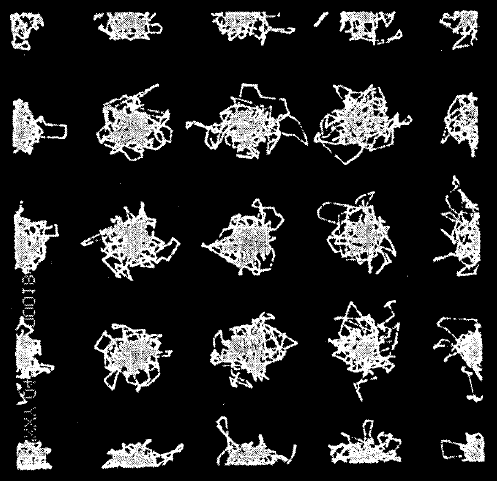
\includegraphics[width=3in]{res1.png}
\end{center}
这是模拟的固态的情形, 可以看到和我们想象的分子运动轨迹还是比较
一致的.
\begin{center}
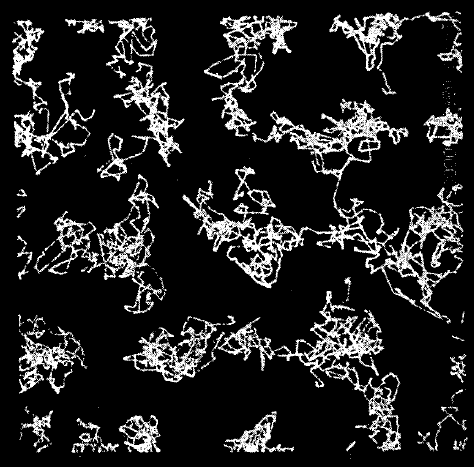
\includegraphics[width=3in]{res2.png}
\end{center}
这是液相的结果, 可以看到分子运动的无规则程度变大了.
\begin{center}
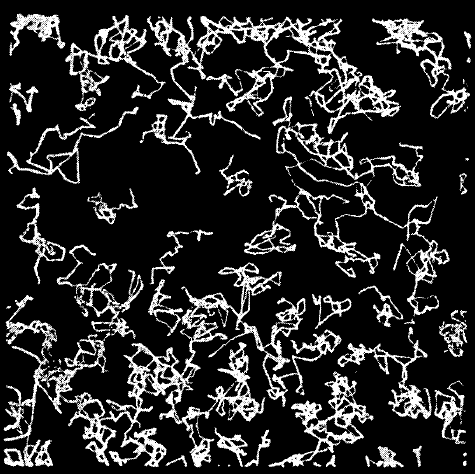
\includegraphics[width=3in]{res3.png}
\end{center}
这是气液混合相的结果, 可以看出这时分子没有一个固定的区域
而是到处乱跑.

\section{方法的局限性}
文献中提出的主要局限是模拟的分子数目过小, 和真实的情况不在
一个数量级上. 这是由于当时计算能力的限制导致的. 还有采用的
势模型 (\ref{potential}) 与真实的情况有所差距. 一个前面
没有提到的细节是在某一步的计算中, 算法采用了周期边界条件,
这在一些系统, 例如发生相变的系统中不一定成立. 最后, 由于
分子动力学的核心思想是积分牛顿方程, 因此这完全是一个经典
的理论, 一切量子效应都是其不能解释的.

\section{应用}
文献最后讨论了这一方法的可能应用. 首先, 前面的结果中也可以
看出, 分子动力学模拟中可以出现气液固相的区别. 因此这种方法
可以用来研究三相的定性性质以及相变过程中的一些细节.

其次, 可以用分子动力学来研究系统在达到平衡态时的一些性质.
例如, 可以用分子动力学来验证 Boltzmann H 定理. 可以得到
系统在各个时刻的速度分布, 这可以用来验证平衡态统计力学.
系统的平均自由程, 自扩散系数, $n$ 点关联函数等等都可以
计算出来.

文章最后说明了这个方向可能的进一步研究. 通过改变系统
的各种参数, 例如边界条件, 势模型, 晶格类型, 大小等,
可以研究各种不同的热力学体系及其性质. 这方面的研究是
一个有价值的方向, 可以发文章.

\end{document}